%!TEX root = theory.tex
% =========================================================================
% -------------------------------------------------------------------------
% Single and Multiphase Flow:
% -------------------------------------------
%
%  This is a good place to outline key objectives of this section.
%
% -------------------------------------------------------------------------

% bold symbols
\def\bnabla{{\boldsymbol{\nabla}}}
\def\bg{{\boldsymbol{g}}}
\def\bq{{\boldsymbol{q}}}
\def\bx{{\boldsymbol{x}}}
\def\bJ{{\boldsymbol{J}}}
\def\K{{\mathbb K}}

% abbreviations
\def\Frac{\displaystyle \frac}

% units
\def\ucdot{{\,\cdot\,}}
\def\ukg{{\rm kg}}
\def\um{{\rm m}}
\def\us{{\rm s}}
\def\umol{{\rm mol}}
\def\upa{{\rm Pa}}

\section{Isothermal Flow Processes}         
\label{sec:flow-processes}

\subsection{Overview}

Subsurface flow simulations typically assume that Darcy's law is valid. 
As this law gives a relationship between velocity and pressure,
it essentially replaces the momentum equation. 
There has been much research to support the validity of Darcy's
Law~\citep{bear-1972}.
Most references give the applicability of Darcy's Law to be 
for laminar flows with Reynolds numbers less that 10 using the pore throat diameter for a soil.
There has been some effort to include inertial as well as turbulence effects that can occur near the wells.

It is also assumed that thermodynamic equilibrium (mechanical and thermal) exists for each grid block.  
Sub-grid scale features often play a prominent role in multi-fluid simulations. 
Faults and fractures will likely be fast paths for contaminant transport and can
effectively be treated with multiple porosity models. 
Similarly, rate-limited diffusion from clay inclusions can also be modeled with a
multiple porosity material.


%%%%%%%%%%%%%%%%%%%%%%%%%%%%%%%%%%%%%%%%%%%%%%%%%%%%%%%%%%%%%%%%%%%%%%%%%%%%%%%%%%%%
%%%%%%%%%%%%%%%%%%%%%%%%%%%%%%%%%%%%%%%%%%%%%%%%%%%%%%%%%%%%%%%%%%%%%%%%%%%%%%%%%%%%

\subsection{Fully Saturated Flow}
\label{sec:flow-single-phase}

The most basic flow model is a single-phase fully saturated flow in a porous medium.  
Notwithstanding its simplicity, it has a wide application to
describing subsurface processes.


%%%%%%%%%%%%%%%%%%%%%%%%%%%%%%%%%%%%%%%%%%%%%%%%%%%%%%%%%%%%%%%%%%%%%%%%%%%%%%%%%%%%
\subsubsection{Assumptions and Applicability}

There are many assumptions required for the strict validity of Darcy's Law, 
including 
\begin{itemize}
\item
  incompressibility and 
\item
  laminararity of the flow.
\end{itemize}
We also assume that 
\begin{itemize}
\item
  solid/rock is incompressible,
\item 
  fluid viscosity is constant,
\item
  there are no fractures, only pores.
\end{itemize}

%%%%%%%%%%%%%%%%%%%%%%%%%%%%%%%%%%%%%%%%%%%%%%%%%%%%%%%%%%%%%%%%%%%%%%%%%%%%%%%%%%%%
\subsubsection{Process Model Equations}

Under the above assumptions fully saturated flow is governed by 
\begin{subequations}
\label{eq:Darcy fully saturated}
\begin{align}
  \phi \left(\Frac{S_s}{g} + \Frac{S_y}{L\,g}\right) \frac{\partial p_l}{\partial t} 
  &=
  -\boldsymbol{\nabla} \cdot (\rho_l \boldsymbol{q}_l) + Q,
  \\
  \bq_l &= -\frac{\K}{\mu_l} 
  (\bnabla p_l - \rho_l \bg),
\end{align}
\end{subequations}
where the primary variable is the fluid presure $p_l$ [\upa]. 
The fluid velocity $\bq_l$ [$\um\ucdot\us^{-1}$] is the dependent variable.
All the other variables can be treated as material parameters
that sometimes may depend on pressure.
These include:
$\phi$ [-] is the porosity,
$S_s$ [$\um^{-1}$] and $S_y$ [-] are specific storage and yeild, respectively,
$g$ [$\um\ucdot\us^{-2}$] is the gravitational constant
and $\bg$ [$\um\ucdot\us^{-2}$] is the gravitational vector,  
$L$ [$\um$] is a characteristic size of the yield layer, 
$\K$ [$\um^2$] is an absolute permeability tensor, and 
$Q$ [$\ukg \ucdot \um^{-3} \ucdot \us^{-1}$] is source or sink term.
 

It is common to see the Darcy Law written in terms of hydraulic head $h$
and the hydraulic conductivity tensor $\K_h$:
\begin{subequations}  \label{eq:HydraulicHead}
\begin{align}
  \bq_l &= -\K_h \bnabla h,
  \\
  h \, &=  z + \frac{p_l}{\rho_l g},
  \\
  \K_h &= \K \, \frac{\rho_l g}{\mu_l}.
\end{align}
\end{subequations}

%%%%%%%%%%%%%%%%%%%%%%%%%%%%%%%%%%%%%%%%%%%%%%%%%%%%%%%%%%%%%%%%%%%%%%%%%%%%%%%%%%%%
\subsubsection{Boundary conditions}


Three types of \textit{boundary conditions} are supported by the model:
\begin{enumerate}
\item
  prescribed pressure $p_l$ (or head), see \eqref{eq:BC pressure};
\item
  prescribed flux, i.e. normal component of the velocity $\bq_l$, see \eqref{eq:BC flux};
\item
  semipervious boundary, see \eqref{eq:BC semipervious}. 
\end{enumerate}
%\citep[for reference see][]{bear-1979}.
These boundary conditions are described in Section~\ref{sec:flow-boundary-conditions}.


\clearpage

%%%%%%%%%%%%%%%%%%%%%%%%%%%%%%%%%%%%%%%%%%%%%%%%%%%%%%%%%%%%%%%%%%%%%%%%%%%%%%%%%%%%
%%%%%%%%%%%%%%%%%%%%%%%%%%%%%%%%%%%%%%%%%%%%%%%%%%%%%%%%%%%%%%%%%%%%%%%%%%%%%%%%%%%%

\subsection{Partially Saturated Flow}
\label{sec:richards-equation}

The Richards equation is often used to describe single phase flow under partially 
saturated conditions (i.e., the pores are not occupied exclusively by a single phase).  
As such, it requires the introduction of a relative permeability and a capillary 
pressure relations. % as discussed in Section~\ref{sec:pc_s_relations}.
The Richards equation is well suited to very large numerical problems (millions of 
degrees of freedom) because it requires only one independent variable per cell.


%%%%%%%%%%%%%%%%%%%%%%%%%%%%%%%%%%%%%%%%%%%%%%%%%%%%%%%%%%%%%%%%%%%%%%%%%%%%%%%%%%%%
\subsubsection{Assumptions and Applicability}

The Richards equation makes the fundamental assumption that 
we are neglecting the movement of the gas phase.
Because of this assumption, using the Richards equation may limit the kinds of 
transport analysis that can be done.
It should also be noted that the Richards equation is often highly nonlinear
due to strong dependence of the relative permeability of the liquid phase
on the liquid saturation.
We also assume that there are no fractures and the water flows through the pores only. 


%%%%%%%%%%%%%%%%%%%%%%%%%%%%%%%%%%%%%%%%%%%%%%%%%%%%%%%%%%%%%%%%%%%%%%%%%%%%%%%%%%%%
\subsubsection{Process Model Equations} 
\label{sec:richards-model-equations}

The Richards equation is derived from the conservation of
liquid mass equation.
In the mixed formulation it is written
for the volumetirc water content $\theta$ [$\umol\ucdot\um^{-3}$] 
and the Darcy velocity $\bq_l$ [$\um\ucdot\us^{-1}$]:  
\begin{subequations}\label{eq:Darcy}
\begin{align}
  \frac{\partial \theta(p_l)}{\partial t} 
  &= 
  -\bnabla \cdot (\eta_l \bq_l) + Q,
  \\
  \bq_l 
  &= 
  -\frac{\K k_{rl}}{\mu_l} (\bnabla p_l - \rho_l \bg),
\end{align}
\end{subequations}
where 
$\eta_l$ [$\umol\ucdot\um^{-3}$] is the molar liquid density,
$Q$ [$\ukg \ucdot \um^{-3} \ucdot \us^{-1}$] is source or sink term,
$\K$ [$\um^2$] is absolute permeability tensor,
$\mu_l$ [$\upa\ucdot\us$ ] is liquid viscosity,
$\rho_l$ [$\ukg\ucdot\um^{-3}$ ] is liquid density, and
$k_{rl}$ [-] is relative permeability.
The total volumetric water content $\theta$ is defined as
a product of porosity $\phi$, molar liquid density $\eta_l$ and liquid saturation $s_l$:
$$
  \theta(p_l) = \phi(p_l) \eta_l\, s_l(p_c).
$$
Usage of the molar liquid density $\theta$
allows us to easily extend the model to a non-isothermal case.

Just like in the case of the fully saturated flow \eqref{eq:Darcy fully saturated},
the primary dependent variable in \eqref{eq:Darcy} is liquid pressure $p_l$.
The difference with \eqref{eq:Darcy fully saturated}
is in that the pressure enters the equations in a nonlinear form,
through a dependence $\theta_l(p_l)$ to be discussed in the following sections.

In general the porosity $\phi$ is a functions of pressure $p_l$.
The relative permeability $k_{rl}$ is a function of saturation $s_l$,
which in turns is a function of capillary pressure $p_c$. 
The relation between pressures $p_l$ and $p_c$ will be discussed in the next section.
Typical models of relative permeability are 
the van Genuchten-Mualem relations \eqref{eq:krl_vGM} and 
the Brooks-Corey-Burdine relations \eqref{eq:krl_BCB}.
The equation \eqref{eq:Darcy} is continuous when transitioning from the saturated to the vadoze zones.

%%%%%%%%%%%%%%%%%%%%%%%%%%%%%%%%%%%%%%%%%%%%%%%%%%%%%%%%%%%%%%%%%%%%%%%%%%%%%%%%%%%%
\subsubsection{Boundary conditions}  

Four types of boundary conditions are supported by the model:
\begin{enumerate}
\item
  prescribed pressure $p_l$ (or head), see \eqref{eq:BC pressure};
\item
  prescribed flux, i.e. normal component of the velocity $\bq_l$, see \eqref{eq:BC flux};
\item
  semipervious boundary, see \eqref{eq:BC semipervious}; %\citep[for reference see][]{bear-1979};
\item
  seepage face.
\end{enumerate}
These boundary conditions are described in Section~\ref{sec:flow-boundary-conditions}.


%%%%%%%%%%%%%%%%%%%%%%%%%%%%%%%%%%%%%%%%%%%%%%%%%%%%%%%%%%%%%%%%%%%%%%%%%%%%%%%%%%%%
\subsubsection{Capillary Pressure -- Saturation Relations}  
\label{sec:richards-pc_s_relations}

Richards equation for unsaturated flow
%, as well as more general multiphase flow models, 
requires representations of the capillary pressure $p_c$ and the relative permeability $k_{rl}$.  
The capillary pressure is a fundamental dependent variable in the multi-phase flow model, and
relates the difference in pressure across an interface between two
fluids to the tendency of a porous medium to pull in the wetting fluid
and push out the non-wetting one.
For the partially saturated fluid flow model typically used to
characterize air-water systems, 
there is only a single capillary pressure:
\begin{equation} \label{eq:GasLiquidCapillaryPressure}
  p_c = p_g - p_l
\end{equation}
where $p_g$ is the pressure of the air/gas. 

Let us define the effective liquid saturation $s_e$ as
\begin{equation}
\label{eq:SaturationDefinition}
s_e \eq \frac{s_l^{} - s_l^r}{s_l^0 - s_l^r}, 
\end{equation}
where $s_l^0$ is the maximum and
$s_l^r$ is the residual (i.e. minimum) liquid saturations. 
Notice that \eqref{eq:SaturationDefinition} implies the effective saturation $s_e$
takes values in the range from zero to one.

Using these definitions, 
two widely used capillary pressure-saturation model relations are presented below, 
namely the Brooks-Corey \citep{brooks1964hydraulic} and van Genuchten \citep{van1980closed} 
models.


\paragraph{Brooks-Corey model.}
The Brooks-Corey form of the saturation function \citep{brooks1964hydraulic} is given by
\begin{equation}
  \label{eq:BC_s_pc_relation}
  s_e \eq \left( \alpha |p_c| \right)^{-\lambda}, 
\end{equation}
where the empirical parameters $\lambda$ [-], and $\alpha$ [$\upa^{-1}$] 
are fit to experimental observations.
The inverse relation is written as
\begin{equation}
  \label{eq:BC_pc_s_relation}
  p_c \eq \frac{1}{\alpha} s_e^{-1/\lambda}.
\end{equation}

\paragraph{Van Genuchten model.}
In the \citet{van1980closed} model the effective liquid saturation is
described by the relation
%
\begin{equation}  
  \label{eq:vG_s_pc_relation}
  s_e \eq \left[1+\left( \alpha |p_c| \right)^n \right]^{-m}, 
\end{equation}
%
with inverse relation
\begin{equation}
  \label{eq:vG_pc_s_relation}
  p_c \eq \frac{1}{\alpha} \left[ s_e^{-1/m} -1 \right]^{1/n}.
\end{equation}
%
The non-dimensional constants $n$ [-], $m$ [-] and dimensional $\alpha$ [$\upa^{-1}$] are
empirical parameters.


One may notice that Van Genuchten model is an evolution of Brooks-Corey model as evident 
both by the dates and the form of the equations.
In particular notice that if we take 
$\lambda = mn$ and $(\alpha p_c)^n \gg 1$, 
then the Brooks-Corey and van Genuchten saturation functions, 
Equations \eqref{eq:BC_s_pc_relation} and \eqref{eq:vG_s_pc_relation}, are equivalent.


%%%%%%%%%%%%%%%%%%%%%%%%%%%%%%%%%%%%%%%%%%%%%%%%%%%%%%%%%%%%%%%%%%%%%%%%%%%%%%%%%%%%
\subsubsection{Relative Permeability -- Saturation Relations}
\label{sec:richards-relative-permeability}

Given capillary pressure - saturation relations $p_c(s_l$, 
the relative permeability relations needed by Richards equation can be defined.  
Two popular relative permeability - saturation relations used in air-water 
systems are the \citet{mualem1976new} and \citet{burdine1953relative} models.
The relative permeability model proposed by \citet{mualem1976new} has the form
\begin{equation} \label{eq:Mualem}
  k_{rl}(s_l) 
  = 
  s_e^{\ell} \, 
  \frac{ \left\{ \displaystyle\int_0^{s_e} p_c(s)^{-1} ds \right\}^2 }
  { \left\{ \displaystyle\int_0^{1} p_c(s)^{-1} ds \right\}^2 },
\end{equation}
where the power $\ell$ in $s_e^\ell$ is a pore-connectivity parameter that varies 
depending on the soil. 
Although, \citet{mualem1976new} estimated an average value of
$\ell=1/2$, values of $\ell$ ranged from -5 to +5 across soils. More recent studies
[cf. \citet{vanG_retc_1991}] have suggested that $\ell=1/2$ may be
appropriate for coarse-textured soils, but not for many medium- and
fine-textured soils. Thus, $\ell$ should be available as a fitting parameter.

Similarly, the older \citet{burdine1953relative} model is given by
\begin{equation}
\label{eq:Burdine}
  k_{rl}(s_l) = s_e^{\ell} \, 
    \frac{ \displaystyle\int_0^{s_e} p_c(s)^{-2} ds }
         { \displaystyle\int_0^{1} p_c(s)^{-2} ds },
\end{equation}
where \citet{burdine1953relative} assumed $\ell=2$. However, as with
the Mualem model \eqref{eq:Mualem}, $\ell$, should be available as a
fitting parameter.


\paragraph{Van Genuchten relative permeability.}
To obtain a closed-form solution for the relative permeability using
either the Mualem or Burdine models (Eqns.\eqref{eq:Mualem} and
\eqref{eq:Burdine}, respectively) combined with the van Genuchten
saturation function, the parameters $n$ and $m$ must be related by the
expressions
\begin{equation}
\label{eq:lambda} 
m = \left\{
  \begin{array}{ll}
    1 - \dfrac{1}{n}, & \text{Mualem},\\[9pt]
    1 - \dfrac{2}{n}, & \text{Burdine}.
  \end{array}
\right.
\end{equation}
In the more general case of independent values of $m$ and $n$ the
relative permeability involves the incomplete beta function \citep{vangenuchten1985}. 
More recently \citep{douradoneto2011} presented a general model for Mualem and 
Burdine relative permeability functions for use with the van Genuchten saturation 
function in terms of hypergeometric functions.


The Burdine relative permeability function for the liquid phase derived
from the van Genuchten saturation function is given by
\begin{equation}
  k_{rl} \eq s_e^{2} \left\{ 1 - \left[ 1 - s_e^{1/m} \right]^m \right\}.
  \label{eq:krl_vGB} 
\end{equation}

The Mualem 
relative permeability function has the form (note power 2):
\begin{equation}
  k_{rl} \eq s_e^{\ell} \left\{ 1 - \left[ 1 - s_e^{1/m} \right]^m \right\}^2.
  \label{eq:krl_vGM} 
\end{equation}




\paragraph{Brooks-Corey relative permeability.}
Combined with the Brooks-Corey saturation function, the Mualem
relative permeability function is given by
\begin{equation} \label{eq:krl_BCM}
  k_{rl} = \big(s_e\big)^{\ell+2+2/\lambda} 
         = \left(\alpha |p_c|\right)^{-((\ell+2)\lambda+2)}.
\end{equation}
The Burdine form originally considered by \citet{brooks1964hydraulic}
is given by
\begin{equation} \label{eq:krl_BCB}
  k_{rl} = \left( s_e \right)^{ \ell+1+2/\lambda}
         = \left( \alpha |p_c| \right)^{-((\ell+1)\lambda+2)}.
\end{equation}


%%%%%%%%%%%%%%%%%%%%%%%%%%%%%%%%%%%%%%%%%%%%%%%%%%%%%%%%%%%%%%%%%%%%%%%%%%%%%%%%%%%%
%%%%%%%%%%%%%%%%%%%%%%%%%%%%%%%%%%%%%%%%%%%%%%%%%%%%%%%%%%%%%%%%%%%%%%%%%%%%%%%%%%%%
%\subsection{Thermal Richards Equation}
%\label{sec:thermal-richards-equation}


%%%%%%%%%%%%%%%%%%%%%%%%%%%%%%%%%%%%%%%%%%%%%%%%%%%%%%%%%%%%%%%%%%%%%%%%%%%%%%%%%%%%
%\subsubsection{Process Model Equations} 

%\begin{equation}
%  \frac{\partial \theta}{\partial t} 
%  =
%  - \bnabla \cdot (\eta_l \bq_l)
%  - \bnabla \cdot (\K_g \bnabla \big(\frac{p_v}{p_g}\big)) + Q,
%  \qquad
%  \bq_l = -\frac{\K k_r}{\mu} (\bnabla p - \rho_l \bg)
%\end{equation}


\clearpage

%%%%%%%%%%%%%%%%%%%%%%%%%%%%%%%%%%%%%%%%%%%%%%%%%%%%%%%%%%%%%%%%%%%%%%%%%%%%%%%%%%%%
%%%%%%%%%%%%%%%%%%%%%%%%%%%%%%%%%%%%%%%%%%%%%%%%%%%%%%%%%%%%%%%%%%%%%%%%%%%%%%%%%%%%
\subsection{Isothermal Richards Equation with Dual Porosity Model}
\label{sec:dual-porosity-richards-equation}

Dual porosity model is designed to model fluid flows
when the solid contains both pores/matrix and fractures.







%%%%%%%%%%%%%%%%%%%%%%%%%%%%%%%%%%%%%%%%%%%%%%%%%%%%%%%%%%%%%%%%%%%%%%%%%%%%%%%%%%%%
\subsubsection{Assumptions and Applicability} 


Typically flow in the fracture is much faster that that in the pores/matrix.
Therefore, 
dual-porosity model assumes that water flow is restricted to the fractures.
The pores in the solid represent immobile pockets that can exchange, retain and store water
but do not permit convective flow.
This leads to dual-porosity type flow and transport models that partition the liquid
phase into mobile and immobile regions.


%%%%%%%%%%%%%%%%%%%%%%%%%%%%%%%%%%%%%%%%%%%%%%%%%%%%%%%%%%%%%%%%%%%%%%%%%%%%%%%%%%%%
\subsubsection{Process Model Equations} 

The Richards equation in the mobile (fracture dominated) region is augmented by the water exchange
term $\Sigma_w$: 
\begin{subequations}
\begin{align}
  \frac{\partial \theta_f}{\partial t} 
  &= 
  -\bnabla \cdot (\eta_l \bq_l) + Q_f - \Sigma_w, 
  \\
  \bq_l 
  &= 
  -\frac{\K k_r}{\mu} (\bnabla p_l - \rho_l \bg),
\end{align}
\end{subequations}
where $\Sigma_w$ is the transfer rate for water from the matrix to the fracture, 
and $Q_f$ is source or sink term [$\ukg \ucdot \um^{-3} \ucdot \us^{-1}$].
The equation for water balance in the matrix is
$$
  \frac{\partial \theta_m}{\partial t} 
  = Q_m + \Sigma_w,
$$
where and $Q_m$ is source or sink term [$\ukg \ucdot \um^{-3} \ucdot \us^{-1}$].
The volumetric water contents $\theta_f$ and $\theta_m$ are defined as
$$
  \theta_f = \phi_f\, \eta_l\, s_{lf},\qquad
  \theta_m = \phi_m\, \eta_l\, s_{lm},
$$
where saturations $s_{lf}$ and $s_{lm}$ may use different 
capillary pressure-saturation models.
The rate of water transfer from the matrix to the fracture regions $\Sigma_w$ 
is proportional to the difference in hydraulic heads:
$$
  \Sigma_w = \alpha_w (h_f - h_m),
$$
where $\alpha_w$ is the mass transfer coefficient.
Since hydraulic heads are needed for both regions, this equation requires
estimating retention curves for both regions and therefore is nonlinear.


%%%%%%%%%%%%%%%%%%%%%%%%%%%%%%%%%%%%%%%%%%%%%%%%%%%%%%%%%%%%%%%%%%%%%%%%%%%%%%%%%%%%
%%%%%%%%%%%%%%%%%%%%%%%%%%%%%%%%%%%%%%%%%%%%%%%%%%%%%%%%%%%%%%%%%%%%%%%%%%%%%%%%%%%%
\subsection{Boundary conditions}
\label{sec:flow-boundary-conditions}


To facilitate the discussion on boundary conditions, consider the case of 
flow described in Fig.~\ref{fig:bc_flow}. 
Although the figure represents a two-dimensional flow field, the passage to three dimensions 
is straightforward and requires no further explanations. 

\begin{figure}  [h]
\begin{center} 
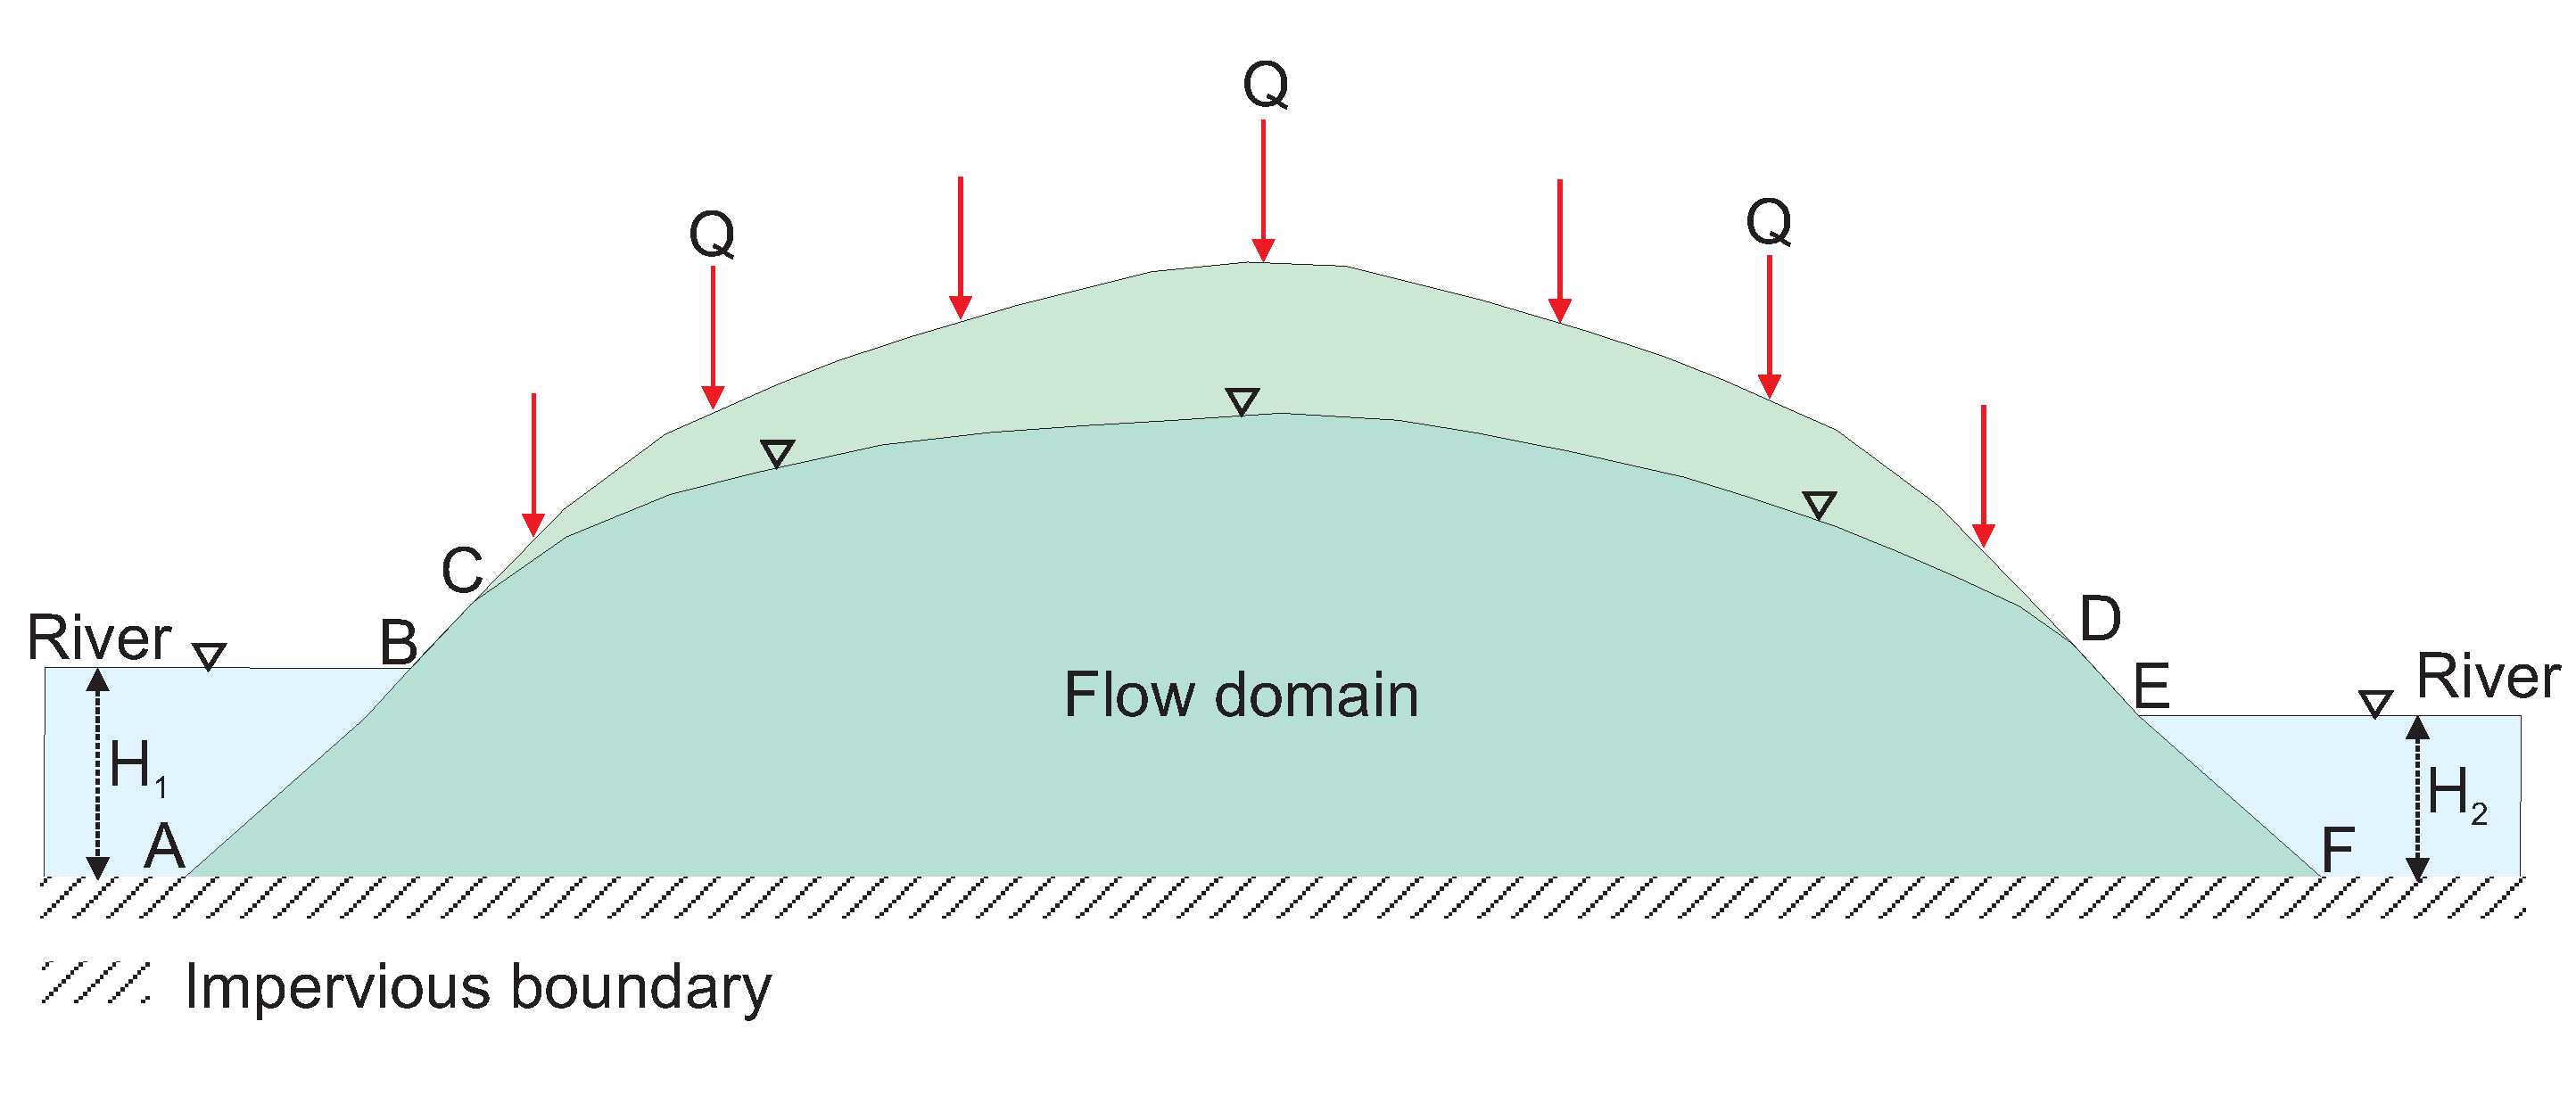
\includegraphics[scale=0.25]{figs/bc_flow.pdf}
\caption{Flow domain between two rivers \citep[it was partially based on]{bear-1972}.}
\label{fig:bc_flow}
\end{center}
\end{figure}

\paragraph{Boundary of prescribed pressure or head.}
This involves the specification of a fixed pressure or hydrostatic head on boundary $\Gamma_D$.
For instance, a boundary of this kind occurs whenever the flow domain is adjacent to a body of open water.
Segments A-B and E-F in Fig.~\ref{fig:bc_flow} are examples of a boundary of prescribed potential.
The pressure or head boundary conditions are given functions, e.g.
\begin{equation}
\label{eq:BC pressure}
  p_l(\bx,t) = p_{b}(\bx,t), \quad \bx \in \Gamma_D. 
\end{equation}

\paragraph{Boundary of prescribed flux.}
This involves the specification of the flux normal to the boundary $\Gamma_N$
(see segment C-D in Figure \ref{fig:bc_flow}):
\begin{equation}
\label{eq:BC flux}
  \bq_l\cdot \bn = q_{b}(\bx,t), \quad \bx \in \Gamma_N,
\end{equation}
where $q_b$ [$\um\ucdot\us^{-1}$] is the given boundary flux. 
For infiltration at the top horizontal surface, it equals to the Darcy velocity
and referred to as the infiltration velocity.

\paragraph{Semipervious boundary (or mixed boundary condition).}
This boundary condition is more complicated than the first two as it involves a case 
in which local conditions within the computational domain influence the flux in or 
out of the domain.
This type of boundary occurs when the porous medium domain is in contact with 
a body of water continuum (or another porous medium domain, see for instance segments 
A-B and E-F in Fig.~\ref{fig:bc_flow}), however, a relatively thin semipervious layer 
separates the two domains:
\begin{equation}
\label{eq:BC semipervious}
  \bq_l \cdot \bn = I\, \left(p (\bx,t) - p_{b}(\bx,t) \right), \quad \bx \in \Gamma_R.
\end{equation}
where $I$ is an impedance and $p_{b}(\bx,t)$ is the given external pressure.

\paragraph{Seepage face.}
As is shown in Fig.~\ref{fig:bc_flow} (see segments B-C and D-E), seepage face (or surface) 
is always present when a phreatic surface ends at the down-stream external boundary of flow domain.
In this case the phreatic surface is tangent to the boundary of the porous medium at points C and D.
Along a seepage surface, water emerges from the flow domain, trickling downward to the adjacent body of water.

A seepage surface is defined as the boundary 
where water leaves the ground surface and then continues to flow in a thin film along its surface.
Being exposed to the atmosphere, the pressure along the seepage face is equal to the atmospheric pressure 
(i.e. capillary pressure $p_{c}=0$). 

The geometry of the seepage face is known (as it coincides with the boundary of the porous medium), 
except for its limit (points C and D in Figure \ref{fig:bc_flow}) 
which is also lying on the (a priori) unknown phreatic surface.
The location of this point is, therefore, part of the required solution.
In unsteady flow, the location of the upper limit of the seepage face varies with time
and could be simulated in two ways:
\begin{enumerate}
\item Using a dynamic boundary condition that switches from a prescribed pressure boundary condition
to a prescribed flux boundary condition representing the recharge.
\item Combining boundary conditions in a hybrid one to represent the transition recharge/seepage 
surface (e.g. see Fig.~\ref{fig:seepage_bc}).
\end{enumerate}

\begin{figure}  [h]
\begin{center}
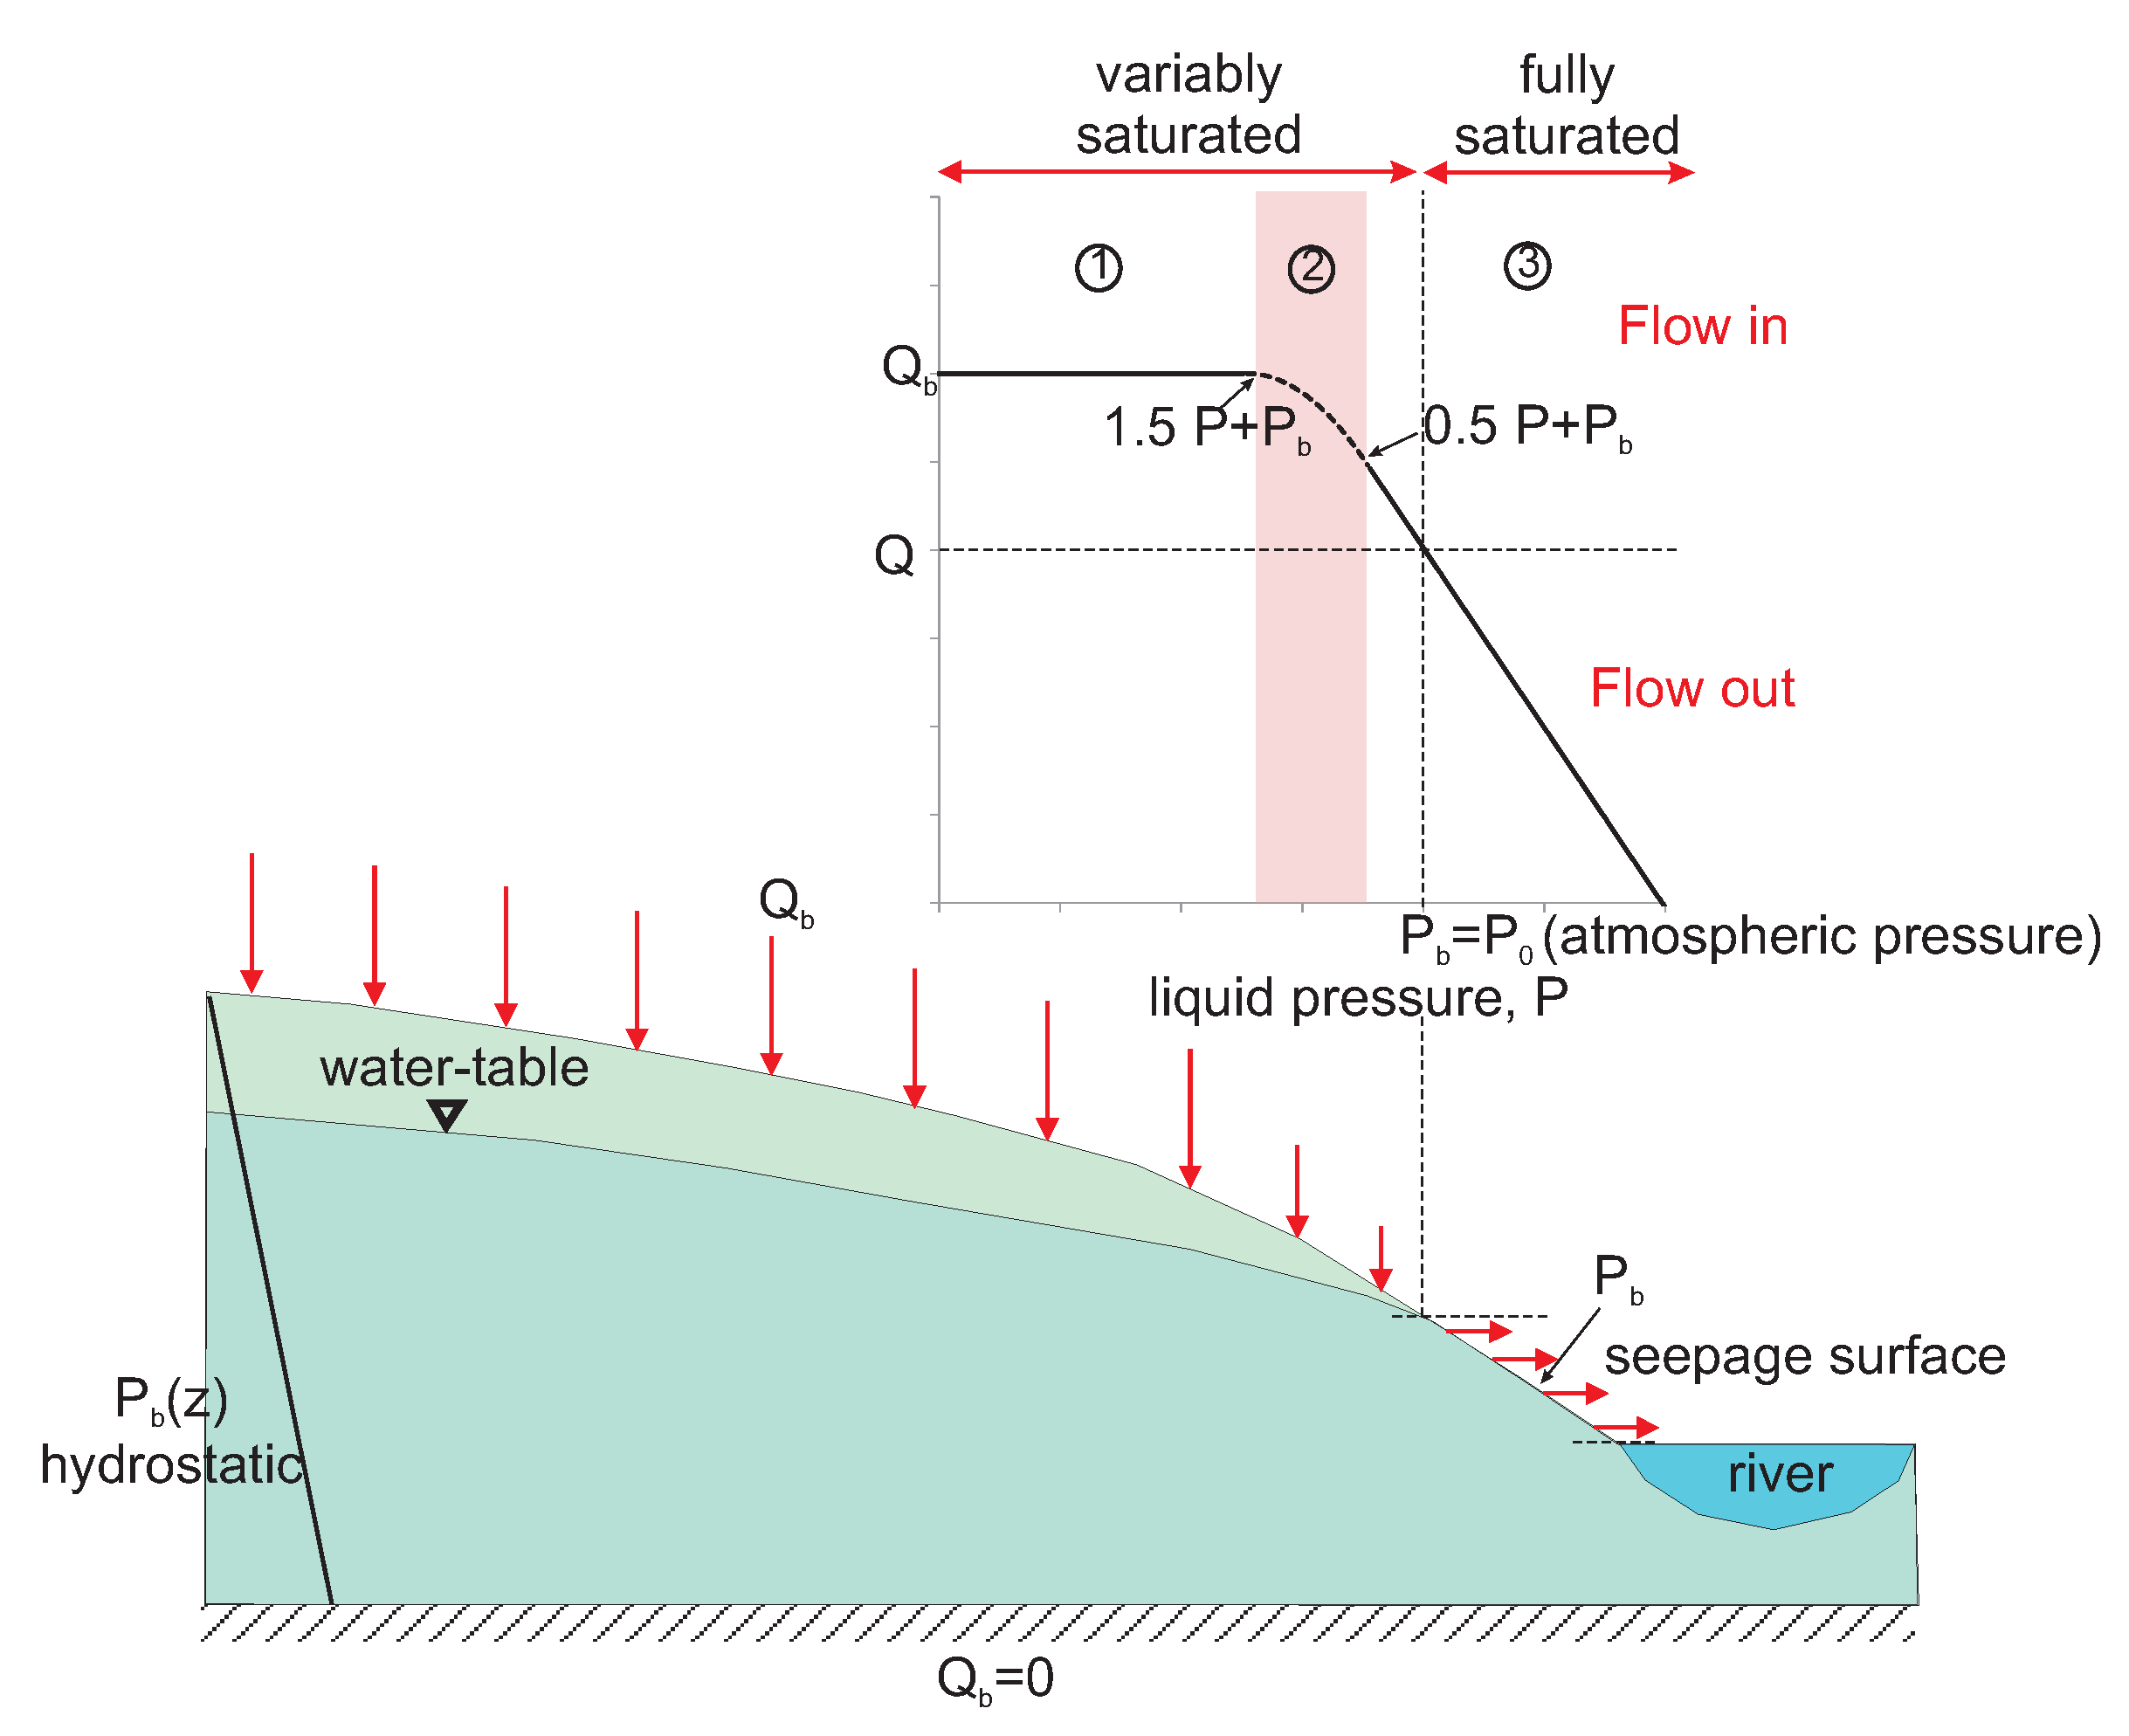
\includegraphics[scale=0.3]{figs/seepage_bc.pdf}
\caption{Seepage face.}
\label{fig:seepage_bc}
\end{center}
\end{figure}

The state of the first option depends on the pressure inside the computational domain.
Regarding the second option, this hybrid boundary condition \citep[based on][]{hamm2000} can be formulated as
\begin{equation} \label{eq:fifth_bc_richard}
\begin{array} {lllll}
  \bq \cdot \bn & = & q_{b}(t) & \qquad \text{for} \quad &  p < \left( \frac{3}{2} p' + p_{0} \right), \\[0.5ex]
  \bq \cdot \bn & = & \frac{\left(  7-2f-f^{2}  \right)}{8} q_{b}(t) 
                    & \qquad \text{for} \quad &  \left( \frac32 p' + p_{0} \right) \leq p \leq \left( \frac12 p' + p_{0} \right), \\[1.0ex]
  \bq \cdot \bn & = & I (p - p_{0}) &  \qquad \text{for} \quad & \left( \frac{1}{2} p' + p_{0} \right) < p, 
\end{array} 
\end{equation}
where $q_{b}(t)$ is the maximum recharge and $f(p,t)$ is a local variable between $-1$ and $1$ 
defined as 
\begin{equation}
  f(p,t) = 2 \frac{p'- (p(x_{b},y_{b},z_{b},t) - p_{0}) }{p'},
\end{equation}
where $p_{0}$ is a reference pressure (in this particular example case, its value is equal to 
the atmospheric pressure), and $p'$ is defined as 
\begin{equation}
  p' = I^{-1} q_{b}(t).
\end{equation}







% =========================================================================
% -------------------------------------------------------------------------
% Infiltration Processes:
% -------------------------------------------
%
%  This is a good place to outline key objectives of this section.
%
% -------------------------------------------------------------------------

\begin{comment}

\subsection{Infiltration} \label{sec:infiltration}
%
%~\todo{This section is called Infiltration but really it 
%       describes the near-surface water balance and recharge. -Freshley}

%\subsubsection{Overview}
%
The infiltration process models are components of the subsurface fluid migration. 
Infiltration can be an important driving force for contaminant transport, especially in the vadose zone.  
Engineered subsurface barrier technology seeks to minimize the infiltration
driving force for contaminant migration.  
There are a number of approaches and models that can be applied to predict infiltration processes. 
These range from simple storage routing models to the more mechanistic 
Richards equation-based 
\todo[color=cyan]{GEH: Suggest that we remove ``Richards equation-based'' and simply say ``more mechanistic models'' 
as Richards equation does not account for heat transport.}
models that simulate water flow and heat transport 
in response to meteorological forcing and plant water uptake. 
Within the complex interaction of physical, hydrologic, and biotic processes 
that control field-scale infiltration at the site of interest, 
the ideal model should be capable of assessing the impact
of infiltration on contaminant transport, 
as well as supporting barrier design and performance assessment.

Predicting infiltration requires consideration of unsaturated flow processes, 
precipitation, surface runoff, water storage,  
lateral diversion along sloped layers, and, ultimately, deep percolation ~\citep{ward_1997,ward_2005}. 
%(Ward and Gee 1997; Ward et al. 2005a). 
All of these processes occur in response to forcing meteorology 
that leads to temporal variability in air temperature, relative humidity, wind speed, and barometric
pressure and, in the most sophisticated implementations, 
require the solution of coupled equations for mass and energy transport.

A minimum set of processes for modeling the water budget should include:  
%
\begin{align}
P + I = R_{over} + \Delta W + D + GD,% + E + T,
\end{align}
where 
$P$ is the precipitation, 
$I$ -- irrigation,
$R_{over}$ -- overland flow (run-off and run-on),
$D$ -- drainage out of the soil cover (diverted by reduced-permeability layer),
$GD$ -- ground water recharge (deep percolation past a reduced-permeability layer), and
$\Delta W$ -- change in soil water storage.
%$E$ = evaporation\\
%$T$ = transpiration.



\noindent 
Evaporation is defined as the process by which liquid water is
transformed into a gaseous state and the subsequent transfer of this
vapor to the atmosphere.  
Transpiration is the loss of water from plants through their stomata to the atmosphere.  
Plants compensate for transpiration losses by taking up water from the soil.

Another requirement is that the process models must include a full energy balance (nonisothermal) option for
evapotranspiration processes.  
Water that does not run off the surface must be available for evaporation from the soil or plant surfaces, 
or infiltration into the soil profile. 
Soil water content must depend on the interactions of precipitation, temperature, vegetation, and albedo changes that vary temporally
(e.g., diurnally, seasonally, and episodically).  
Spatially and temporally variable water storage and flux must be available for contaminant transport.


\subsubsection{Process Model Requirements}

\paragraph{Precipitation. } 
The treatment of precipitation 
%~\todo{Why this limitation? - Finsterle} 
must include all natural sources of moisture that may reach the surface 
in the form of rain, snow, sleet, hail, dew, and fog, and must account for precipitation not available for infiltration. 
This includes precipitation intercepted by the plant canopy, from which it is evaporated
or transpired without ever contacting the soil; and sublimation, the direct conversion of water from the solid phase to the vapor phase.  
This should also account for the presence of a snow cover that can delay
infiltration, reduce evaporation rates, and in the event of rapid snowmelt, lead to surface runoff.

%\subsubsection{Deterministic}

%\subsubsection{Stochastic}

\paragraph{Non-Precipitation Surface Recharge (including leaks).} 
Process models should account for surface recharge sources (e.g., irrigation water used
during construction as a dust control agent and post-construction to
support the establishment of vegetation; water condensing on plant
surfaces and falling to the ground once the maximum storage depth in
the canopy is exceeded, pipe leaks).  
These sources must also be subject to evaporation from soil and plant surfaces with the remainder
becoming available for runoff or infiltration.





% =========================================================================
% -------------------------------------------------------------------------
% Section 3 Data Requirements for Flow
% -------------------------------------------
%
%  Phases, Components, and Variables
%
% -------------------------------------------------------------------------

\subsection{Data Requirements for Flow}

\subsubsection{Permeability and Porosity}

The most basic properties of the subsurface, which are required for
all of the flow models, are permeability and porosity.  Often this
data can only be provided by sparsely located well logs and at a
spatial scale much finer than the scale of the model. As a
consequence, techniques of upscaling are required to fill in the
missing data and extrapolate to larger scales.

Permeability estimates are available for a large variety of soils and
rocks. When conceptual (and numerical) models have cells that
represent fractures or faults, field tests (pumping and/or tracer) are
required to determine effective permeabilities. Porosity data is also
available for many rock and soil types.

\subsubsection{Relative Permeability and Capillary Pressure.}

For both the Richards equation and more general multiphase problems, the
model requires representations of relative permeability and capillary
pressure.  For two-phase systems, relative permeability and capillary
pressure data are widely available for the more common forms such as
van Genuchten and Brooks Corey.

When a NAPL phase is present and the likelihood of three phases is
significant, much of the relative permeability data available from the
soil literature may have only limited applicability and experiments on
at least core size sample will be necessary.
\citet{stone1973estimation} presented a method to estimate three-phase
relative permeability that is in common usage in the oil
industry. However, when fractures or faults are present, parameters of
the relative permeability and capillary pressure models are estimated
with field data.  Relative permeabilities often exhibit strong
hysteretic behavior.  Land's method
\citep{land1968calculation,spiteri2006impact} is one approach for
handling hysteretic behavior that is relatively simple to implement
and is commonly used in the oil industry.

 Some capillary pressure data is available in the database described
by \citet{schaap2001computer}. Capillary models derived using surface
tension data of pure components \citep{prausnitz1977properties} are
used where experimental data is not available.

\subsubsection{Fluid Characterization}

The model equations must also be augmented with property data for the
fluids.  In simple problems we require only estimates of density and
viscosity for each of the flowing phases.  For more complex problems
in which we are modeling a multicomponent system, additional data is
required.

\end{comment}


\begin{comment}
\subsubsection{Boundary Conditions and Initial Conditions}

Boundary and initial conditions can take several different forms
depending on the application. Dirichlet boundary conditions specify
the pressure, temperature, and saturation at the boundary. Neumann
conditions specify the flux $\bq$ at the boundary.  Initial conditions
may consist of specifying a constant pressure or variable pressure,
temperature, and saturation, for example in the form of hydrostatic
conditions taking into account the change in fluid density.

Typical boundary condition for Richard's equation consist of
infiltration (recharge) and constant or time varying pressure
conditions. More sophisticated conditions such at unit gradient, free
drainage, and seepage face are also used.

%
%  Need to fix this with the BC section.
% 

\subsubsection{Boundary Conditions and Initial Conditions}
%------------------------------------------------------------------------------
%------------------------------------------------------------------------------
%------------------------------------------------------------------------------
Boundary conditions for flow are exhaustively detailed in Subsection \ref{sec:bc_flow}. 
They and initial conditions can take several different forms depending on the application. 
Dirichlet boundary conditions specify the pressure, temperature, and saturation at the boundary. 
Neumann conditions specify the flux $\bq$ at the boundary. 
Initial conditions may consist of specifying a constant pressure or variable pressure, temperature, and saturation, for example in the form of hydrostatic conditions taking into account the change in fluid density.
%------------------------------------------------------------------------------
\\
%------------------------------------------------------------------------------
% For Richards equations
%------------------------------------------------------------------------------
Typical boundary conditions for the Richards equation consist of infiltration (recharge) and constant or time varying pressure conditions, but also to impose a prescribed pressure (i.e. Dirichlet boundary condition) is a valid option. 
More sophisticated conditions such at unit gradient, free drainage, and seepage face are also used.
%More sophisticated conditions such at unit gradient and seepage face
%are also used.  For the component (NAPL) fluids, specified mole
%fractions and flowrates (sources/sinks) are usual boundary conditions.
%------------------------------------------------------------------------------
\\
%------------------------------------------------------------------------------
% For multiphase flow 
%------------------------------------------------------------------------------
As regards the multiphase approach, additional data for the boundary and in initial conditions could be required such as the mass fraction for the {\textit{j}}th component in the phase $\alpha$ ($Y_{j \alpha}$, see equation \eqref{eq:MultiphaseConservationEquation}).  
\end{comment}





 






